\documentclass[conference,a4paper]{IEEEtran}
\IEEEoverridecommandlockouts
\usepackage[T1]{fontenc}
\usepackage[utf8]{inputenc}
\usepackage[english,spanish,es-tabla,es-nodecimaldot,es-noshorthands]{babel}
\usepackage{cite}
\usepackage{amsmath,amssymb,amsfonts}
\usepackage{graphicx}
\usepackage{textcomp}
\usepackage{xcolor}
\usepackage{array}
\usepackage{url}
\usepackage{tikz}
\usetikzlibrary{positioning,arrows.meta}

% Estilo IEEE para los nombres de figuras y palabras clave
\addto\captionsspanish{\renewcommand{\figurename}{Fig.}}
\renewcommand{\IEEEkeywordsname}{Palabras clave}

\begin{document}

\title{Billetes Perú: aplicación móvil accesible para el reconocimiento de billetes peruanos en el dispositivo mediante aprendizaje profundo}

\author{\IEEEauthorblockN{Angel Raul Caceres Pari}
\IEEEauthorblockA{\textit{Escuela Profesional de Ingeniería de Sistemas} \\
\textit{Universidad Nacional de San Agustín de Arequipa}\\
Arequipa, Perú \\
acacerespar@unsa.edu.pe}
\and
\IEEEauthorblockN{Francis Willian Ayamamani Añasco}
\IEEEauthorblockA{\textit{Escuela Profesional de Ingeniería de Sistemas} \\
\textit{Universidad Nacional de San Agustín de Arequipa}\\
Arequipa, Perú \\
fayamamani@unsa.edu.pe}
}

\maketitle

\begin{abstract}
Las personas con discapacidad visual tienen dificultades para identificar por sí mismas el valor de los billetes, situación que en el Perú se agrava porque circulan a la vez dos familias de billetes y las marcas táctiles se desgastan con el uso. Este artículo presenta Billetes Perú, una aplicación móvil multiplataforma desarrollada en Flutter que reconoce billetes de S/~10, 20, 50 y 100 con la cámara del teléfono y anuncia su valor mediante voz con estilo de dictado, tonos y vibración, sin requerir conexión a internet. Se entrenó por transferencia de aprendizaje un modelo MobileNetV3-Small con un conjunto público de 9315 imágenes de billetes peruanos y se exportó a TensorFlow Lite con cuantización de rango dinámico (1,13~MB). El modelo cuantizado alcanzó una exactitud de 96,9~\% y un F1 macro de 0,969 en 1237 imágenes de prueba. Con un umbral de confianza de 0,85, la aplicación anuncia un valor en el 94,3~\% de los casos y se equivoca solo en el 0,77~\% de sus anuncios. La aplicación incluye además un sumador con cálculo de vuelto, historial, cuentas locales y ajustes de accesibilidad, y fue verificada en un teléfono Android.
\end{abstract}

\begin{IEEEkeywords}
discapacidad visual, reconocimiento de billetes, aprendizaje profundo, MobileNetV3, TensorFlow Lite, Flutter, accesibilidad.
\end{IEEEkeywords}

{\renewcommand{\abstractname}{Abstract}\renewcommand{\IEEEkeywordsname}{Index Terms}
\begin{otherlanguage*}{english}
\begin{abstract}
Visually impaired people struggle to identify banknote denominations on their own, a problem aggravated in Peru by two banknote families circulating at once and by worn tactile marks. This paper presents Billetes Perú, a cross-platform Flutter mobile app that recognizes S/~10, 20, 50 and 100 notes with the phone camera and announces their value through dictation-style speech, earcons and vibration, fully offline. A MobileNetV3-Small model was trained by transfer learning on a public dataset of 9315 Peruvian banknote images and exported to TensorFlow Lite with dynamic-range quantization (1.13~MB). The quantized model reached 96.9\% accuracy and 0.969 macro F1 on 1237 test images. With a 0.85 confidence threshold, the app speaks in 94.3\% of cases and is wrong in only 0.77\% of its announcements. The app also offers a banknote adder with change calculation, history, local accounts and accessibility settings, and was verified on an Android phone.
\end{abstract}
\begin{IEEEkeywords}
visual impairment, banknote recognition, deep learning, MobileNetV3, TensorFlow Lite, Flutter, accessibility.
\end{IEEEkeywords}
\end{otherlanguage*}}

\section{Introducción}

Según la Organización Mundial de la Salud, al menos 2200 millones de personas en el mundo tienen algún tipo de deficiencia visual o ceguera \cite{who2019}. En el Perú, el Censo Nacional 2017 registró 3\,051\,612 personas con alguna discapacidad (10,3~\% de la población), y la dificultad para ver fue la más frecuente, reportada por el 48,3~\% de ellas \cite{inei2019}. Para este grupo, una tarea cotidiana como pagar o comprobar un vuelto en efectivo depende de poder reconocer el valor de cada billete.

Desde 2021 el Banco Central de Reserva del Perú (BCRP) emite una nueva familia de billetes con elementos táctiles de mayor relieve para personas con discapacidad visual \cite{bcrp2021}, pero esta circula junto con la familia anterior \cite{caytuiro2023}, de diseño y marcas distintas. Además, el relieve se pierde con el desgaste y los billetes suelen estar doblados. Las aplicaciones existentes no cubren bien esta necesidad: Cash Reader reconoce más de 100 monedas, pero su versión gratuita solo identifica las denominaciones más bajas de cada moneda \cite{cashreader}, y hasta 2023 no existía un conjunto de datos etiquetado de billetes peruanos para entrenar modelos propios \cite{caytuiro2023}.

Este trabajo propone \emph{Billetes Perú}, una aplicación móvil que reconoce billetes peruanos con la cámara, ejecuta el modelo dentro del teléfono y comunica el resultado con voz, sonido y vibración.

\subsection{Problema de investigación}

La Fig.~\ref{fig:arbol} resume el análisis del problema mediante un árbol de problemas. El problema central es la dificultad de las personas con discapacidad visual para identificar por sí mismas el valor de los billetes peruanos. Sus causas son técnicas (marcas táctiles desgastadas, dos familias de billetes) y tecnológicas (herramientas de pago, que exigen conexión o no cubren el sol peruano, y escasez de datos locales). Sus efectos son prácticos: dependencia de terceros, riesgo de engaño y menor inclusión financiera.

\begin{figure*}[!t]
\centering
\resizebox{0.92\textwidth}{!}{%
\begin{tikzpicture}[
  caja/.style={draw, rounded corners=2pt, align=center, font=\footnotesize, minimum height=12mm, text width=36mm, inner sep=3pt},
  efecto/.style={caja, fill=orange!14},
  causa/.style={caja, fill=blue!9},
  central/.style={caja, fill=red!14, text width=122mm, font=\small\bfseries, minimum height=11mm},
  flecha/.style={-{Stealth[length=2mm]}, thick}]
\node[central] (P) {Dificultad de las personas con discapacidad visual para identificar\\ por sí mismas el valor de los billetes peruanos};
\node[efecto, above=10mm of P] (E2) {Riesgo de engaño y de pérdidas económicas al pagar o recibir vuelto};
\node[efecto, left=8mm of E2] (E1) {Dependencia de terceros en compras y transacciones cotidianas};
\node[efecto, right=8mm of E2] (E3) {Menor autonomía e inclusión financiera};
\node[causa, below=10mm of P, xshift=-21mm] (C2) {Dos familias de billetes en circulación, con diseños y marcas distintas};
\node[causa, left=4mm of C2] (C1) {Marcas táctiles desgastadas y billetes doblados o arrugados};
\node[causa, below=10mm of P, xshift=21mm] (C3) {Aplicaciones de pago, que requieren internet o no cubren el sol peruano};
\node[causa, right=4mm of C3] (C4) {Pocos datos y modelos entrenados con billetes peruanos};
\foreach \c in {C1,C2,C3,C4} \draw[flecha] (\c) -- (P);
\foreach \e in {E1,E2,E3} \draw[flecha] (P) -- (\e);
\node[font=\scriptsize\bfseries, rotate=90, left=2mm of E1, anchor=south] {EFECTOS};
\node[font=\scriptsize\bfseries, rotate=90, left=2mm of C1, anchor=south] {CAUSAS};
\end{tikzpicture}}
\caption{Árbol de problemas que motiva el proyecto.}
\label{fig:arbol}
\end{figure*}

\subsection{Objetivos}

\textbf{Objetivo general:} desarrollar una aplicación móvil accesible que reconozca billetes peruanos en el dispositivo y comunique su valor por voz a personas con discapacidad visual.

\textbf{Objetivos específicos:}
\begin{enumerate}
\item Entrenar un clasificador ligero de billetes peruanos y evaluarlo con exactitud, precisión, exhaustividad, F1 y matriz de confusión.
\item Exportar el modelo a TensorFlow Lite para ejecutarlo sin conexión dentro del teléfono.
\item Diseñar una salida de voz clara, con estilo de dictado, que evite anuncios erróneos mediante un umbral de confianza.
\item Implementar en Flutter una aplicación con reconocimiento, sumador con vuelto, historial, cuentas y ajustes, usable con y sin lector de pantalla.
\end{enumerate}

\subsection{Antecedentes}

Caytuiro-Silva \emph{et al.}~\cite{caytuiro2023,mendeley2023} publicaron el primer conjunto de datos etiquetado de billetes peruanos: 9315 fotografías tomadas con celulares de las dos familias de billetes de S/~10, 20, 50 y 100, con fondos e iluminaciones variadas, pero sin modelos entrenados de referencia. En otros países, Mushtaq \emph{et al.}~\cite{mushtaq2025} reconocieron billetes paquistaníes para personas ciegas con YOLOv8 (99,1~\% de exactitud); Ghanem \emph{et al.}~\cite{ghanem2025} compararon YOLOv8, YOLOv9 y YOLOv10 con billetes egipcios (F1 de 0,9715 con YOLOv10), sin evaluarlos en un teléfono; y Shreya \emph{et al.}~\cite{shreya2025} combinaron un YOLOv8 nano modificado con retroalimentación por voz para dólares, euros y takas (97,73~\% de exactitud). BankNote-Net~\cite{oviedo2022} propone un conjunto abierto de 24\,826 imágenes de 17 monedas para tecnologías de asistencia, con un codificador MobileNetV2. En cuanto a técnicas, este trabajo se apoya en MobileNetV3~\cite{howard2019}, diseñada para teléfonos; en la transferencia de aprendizaje desde ImageNet~\cite{yosinski2014,deng2009}; y en la cuantización de redes para inferencia eficiente~\cite{jacob2018}.

\subsection{Preguntas de investigación e hipótesis}

\begin{itemize}
\item \textbf{PI1:} ¿Puede un modelo de menos de 2~MB, ejecutable en el teléfono, clasificar las cuatro denominaciones con exactitud alta?
\item \textbf{PI2:} ¿Puede un umbral de confianza combinado con votación temporal reducir los anuncios erróneos a un nivel aceptable?
\end{itemize}

\textbf{H1:} el modelo cuantizado alcanza una exactitud de al menos 95~\% en el conjunto de prueba. \textbf{H2:} con un umbral de 0,85, menos del 1~\% de los valores anunciados son erróneos.

\subsection{Aclaraciones terminológicas}

\textbf{Transferencia de aprendizaje:} reutilizar una red preentrenada en otra tarea (aquí, ImageNet) y entrenar solo su parte final. \textbf{Ajuste fino:} reentrenar después toda la red con una tasa de aprendizaje baja. \textbf{TensorFlow Lite (LiteRT):} formato y motor de Google para ejecutar modelos en dispositivos móviles~\cite{litert}. \textbf{Cuantización de rango dinámico:} guardar los pesos en enteros de 8 bits para reducir el tamaño del modelo. \textbf{TTS:} síntesis de texto a voz. \textbf{Lector de pantalla:} software que lee en voz alta la interfaz (TalkBack en Android, VoiceOver en iOS).

\section{Métodos}

\subsection{Naturaleza y enfoque del proyecto}

Se trata de una investigación aplicada con enfoque cuantitativo. El desarrollo siguió cinco fases iterativas: 1) análisis del problema y de requerimientos; 2) preparación de datos; 3) entrenamiento y evaluación del modelo; 4) diseño e implementación de la aplicación; y 5) pruebas fuera de línea y en un dispositivo real.

\subsection{Análisis de requerimientos}

Los requerimientos (Tabla~\ref{tab:req}) se obtuvieron mediante análisis documental de estadísticas y antecedentes~\cite{who2019,inei2019,caytuiro2023}, comparación con soluciones existentes~\cite{cashreader,mushtaq2025,ghanem2025,shreya2025} y las pautas de accesibilidad WCAG~2.2~\cite{wcag22}, en particular las de contraste, tamaño de los objetivos táctiles y compatibilidad con lectores de pantalla.

\begin{table}[!t]
\caption{Requerimientos funcionales (RF) y no funcionales (RNF)}
\label{tab:req}
\centering
\footnotesize
\begin{tabular}{|c|p{6.9cm}|}
\hline
\textbf{ID} & \textbf{Requerimiento} \\
\hline
RF1 & Reconocer en tiempo real la denominación del billete con la cámara trasera. \\
RF2 & Anunciar el valor por voz con estilo de dictado, tono y vibración. \\
RF3 & Sumar billetes, deshacer, reiniciar y calcular lo que falta o el vuelto de un monto a pagar. \\
RF4 & Guardar un historial de reconocimientos por usuario. \\
RF5 & Registrar cuentas, iniciar sesión o entrar como invitado. \\
RF6 & Ajustar voz, sonidos, vibración, linterna y nivel de confianza. \\
RF7 & Ofrecer ayuda hablada. \\
\hline
RNF1 & Funcionar sin conexión a internet (inferencia en el dispositivo). \\
RNF2 & Ser usable con TalkBack/VoiceOver y sin ellos; alto contraste y botones grandes. \\
RNF3 & Modelo menor de 5~MB y aplicación menor de 50~MB. \\
RNF4 & No enviar imágenes fuera del teléfono; contraseñas cifradas. \\
RNF5 & Preferir el silencio a un anuncio dudoso (umbral de confianza). \\
RNF6 & Código único para Android e iOS. \\
\hline
\end{tabular}
\end{table}

\subsection{Conjunto de datos}

Se usó el conjunto \emph{Peruvian Banknotes}~\cite{mendeley2023} (licencia CC~BY~4.0). Sus 16 clases (4 denominaciones $\times$ 2 familias $\times$ 2 caras) se agruparon en cuatro clases por valor: \texttt{b10}, \texttt{b20}, \texttt{b50} y \texttt{b100}. Como la carpeta de prueba original (261 imágenes) no incluye etiquetas, el conjunto de validación original se dividió de forma determinista (por \emph{hash} MD5 del nombre de archivo) en una mitad para validación y otra para prueba. La Tabla~\ref{tab:datos} muestra la distribución final.

\begin{table}[!t]
\caption{Distribución de imágenes por clase y partición}
\label{tab:datos}
\centering
\footnotesize
\begin{tabular}{|l|r|r|r|}
\hline
\textbf{Clase} & \textbf{Entrenamiento} & \textbf{Validación} & \textbf{Prueba} \\
\hline
S/~10 (\texttt{b10}) & 1106 & 331 & 316 \\
S/~20 (\texttt{b20}) & 1281 & 392 & 383 \\
S/~50 (\texttt{b50}) & 2307 & 354 & 360 \\
S/~100 (\texttt{b100}) & 1874 & 172 & 178 \\
\hline
\textbf{Total} & \textbf{6568} & \textbf{1249} & \textbf{1237} \\
\hline
\end{tabular}
\end{table}

\subsection{Modelo y entrenamiento}

Se usó MobileNetV3-Small~\cite{howard2019} preentrenada en ImageNet~\cite{deng2009}, sin su clasificador original, seguida de un \emph{pooling} promedio global, \emph{dropout} de 0,3 y una capa densa \emph{softmax} de cuatro salidas. La red incluye su propia normalización, por lo que recibe píxeles en el rango 0--255. Las imágenes se recortaron al cuadrado central y se redimensionaron a $224\times224$, igual que en la aplicación. Para simular orientaciones e iluminaciones distintas se aplicaron aumentos aleatorios de rotación ($\pm180^\circ$), zoom ($\pm20$~\%), brillo y contraste ($\pm40$~\%). Para compensar el desbalance de clases (S/~50 tiene el doble de imágenes que S/~10), cada clase $c$ recibió el peso
\begin{equation}
w_c = \frac{N}{K\, n_c},
\end{equation}
donde $N$ es el total de imágenes de entrenamiento, $K=4$ el número de clases y $n_c$ las imágenes de la clase $c$. El entrenamiento tuvo dos fases (Tabla~\ref{tab:hiper}): primero solo la capa final, con la red base congelada, y luego un ajuste fino de toda la red. Se usó parada temprana sobre la pérdida de validación.

\begin{table}[!t]
\caption{Configuración del entrenamiento}
\label{tab:hiper}
\centering
\footnotesize
\begin{tabular}{|l|l|}
\hline
\textbf{Parámetro} & \textbf{Valor} \\
\hline
Red base & MobileNetV3-Small (ImageNet) \\
Entrada & $224\times224\times3$, píxeles 0--255 \\
Fase 1 & Base congelada, Adam $10^{-3}$, 12 épocas \\
Fase 2 (ajuste fino) & Toda la red, Adam $10^{-5}$, 10 épocas \\
Lote / pérdida & 32 / entropía cruzada categórica \\
Parada temprana & Paciencia 3 sobre la pérdida de validación \\
Pesos por clase & S/10: 1,48; S/20: 1,28; S/50: 0,71; S/100: 0,88 \\
Hardware & Google Colab, GPU NVIDIA T4 \\
Software & TensorFlow 2.21, Keras 3, scikit-learn~\cite{pedregosa2011} \\
\hline
\end{tabular}
\end{table}

El modelo entrenado se exportó con el convertidor de TensorFlow Lite~\cite{abadi2016,litert} usando cuantización de rango dinámico, que guarda los pesos en 8 bits~\cite{jacob2018}. El archivo resultante, \texttt{soles.tflite}, pesa 1,13~MB.

\subsection{Diseño del sistema}

La Fig.~\ref{fig:arq} muestra la arquitectura. La aplicación se desarrolló en Flutter~3.44 (Dart~3.12)~\cite{flutter}, con un solo código para Android e iOS. La cámara entrega cuadros en formato YUV420 (Android) o BGRA (iOS). En un solo recorrido, cada cuadro se recorta al cuadrado central, se reduce a $224\times224$ y se convierte a RGB:
\begin{equation}
\begin{aligned}
R &= Y + 1{,}402\,V', \qquad B = Y + 1{,}772\,U',\\
G &= Y - 0{,}344\,U' - 0{,}714\,V',
\end{aligned}
\end{equation}
con $U' = U-128$ y $V' = V-128$. La inferencia se ejecuta con \texttt{tflite\_flutter} en un \emph{isolate} separado, para no bloquear la interfaz, procesando como máximo un cuadro cada 150~ms. Un estabilizador decide cuándo hablar: sea $\hat{y}_t$ la clase predicha en el cuadro $t$ con confianza $c_t$ y $\tau$ el umbral (0,85 por defecto). La aplicación anuncia $\hat{y}_t$ solo si
\begin{equation}
c_t \geq \tau \ \wedge\ \bigl|\{\, i \in [t-4,\,t] : \hat{y}_i = \hat{y}_t,\ c_i \geq \tau \,\}\bigr| \geq 4,
\end{equation}
y no repite el mismo valor antes de 5~s. Si el brillo medio de los cuadros es bajo durante varios cuadros seguidos, la linterna se enciende sola.

\begin{figure}[!t]
\centering
\resizebox{\columnwidth}{!}{%
\begin{tikzpicture}[
  bloque/.style={draw, rounded corners=2pt, fill=#1, align=center, font=\footnotesize, text width=42mm, minimum height=10mm, inner sep=3pt},
  bloque/.default=gray!8,
  flecha/.style={-{Stealth[length=2mm]}, thick}]
\node[bloque=blue!9] (cam) {\textbf{Cámara trasera}\\ cuadros YUV420 / BGRA};
\node[bloque, below=5mm of cam] (pre) {\textbf{Preprocesamiento}\\ recorte central $224\times224$, RGB};
\node[bloque=orange!14, below=5mm of pre] (inf) {\textbf{Inferencia TFLite} (\emph{isolate})\\ MobileNetV3-Small, 1,13~MB};
\node[bloque, below=5mm of inf] (est) {\textbf{Estabilizador}\\ $c\geq\tau$, 4 de 5 cuadros, 5~s};
\node[bloque=green!12, below=5mm of est] (sal) {\textbf{Salida multimodal}\\ voz con estilo de dictado, tono,\\ vibración y texto grande};
\foreach \a/\b in {cam/pre, pre/inf, inf/est, est/sal} \draw[flecha] (\a) -- (\b);
\draw[flecha, dashed] (pre.west) -- ++(-5mm,0) |- node[pos=0.25, left, font=\scriptsize, align=center] {brillo\\bajo:\\linterna} (cam.west);
\node[bloque=yellow!22, text width=27mm, anchor=north west, minimum height=52mm] (app) at ([xshift=7mm]cam.north east)
  {\textbf{Aplicación Flutter}\\[3pt] Inicio de sesión\\ y registro\\[2pt] Menú accesible\\[2pt] Reconocer\\[2pt] Sumador (vuelto)\\[2pt] Historial\\[2pt] Ajustes y Ayuda};
\node[bloque=gray!14, text width=27mm, below=4mm of app] (dat) {\textbf{Almacenamiento local}\\ cuentas (SHA-256 + sal), historial y ajustes};
\draw[flecha] (est.east) -- (est.east -| app.west);
\draw[flecha] (app) -- (dat);
\end{tikzpicture}}
\caption{Arquitectura de la aplicación: reconocimiento en el dispositivo y módulos de la interfaz.}
\label{fig:arq}
\end{figure}

\textbf{Voz con estilo de dictado.} El motor TTS del sistema (paquete \texttt{flutter\_tts}) elige en este orden el español de Perú, el latinoamericano o el de España. Habla a una velocidad de 0,42 (la normal es 0,5) y con un tono de 0,95, y divide cada mensaje en frases cortas separadas por una pausa de 350~ms, por ejemplo: «Sumé veinte soles.» — «Total: setenta soles.». Los montos se convierten a palabras en español (por ejemplo, «veintiún soles» o «tres soles con cincuenta céntimos»), para que se pronuncien bien. Antes de cada anuncio suena un tono breve, distinto para detección, suma y aviso, acompañado de vibración, y cada mensaje nuevo interrumpe al anterior para que la aplicación nunca hable con retraso.

\textbf{Interacción accesible.} La interfaz usa amarillo (\#FFD600) sobre negro, con un contraste de aproximadamente 14,9:1 (WCAG exige 7:1 para el nivel AAA~\cite{wcag22}), y botones de al menos 84~dp de alto. Sin lector de pantalla, el primer toque sobre un botón dice qué hace y el segundo, dentro de 3~s, lo activa. Con TalkBack o VoiceOver activos se respetan sus gestos nativos. En las pantallas de cámara, tocar en cualquier parte repite el último valor (Reconocer) o suma el billete detectado (Sumador).

\textbf{Módulos.} El \emph{Sumador} acumula los montos en céntimos (enteros, para evitar errores de redondeo) y, si se indica un monto a pagar, anuncia cuánto falta o el vuelto. El \emph{Historial} guarda hasta 300 registros por usuario. Las \emph{cuentas} son locales: la contraseña se guarda como SHA-256 con una sal aleatoria de 16 bytes. Ninguna imagen sale del teléfono.

\subsection{Pruebas y experimentos}

\begin{enumerate}
\item \textbf{Evaluación fuera de línea} del archivo \texttt{.tflite} final (el mismo que usa la aplicación) sobre los conjuntos de prueba y validación, con las métricas
\begin{equation}
P=\tfrac{TP}{TP+FP},\quad R=\tfrac{TP}{TP+FN},\quad F_1=\tfrac{2PR}{P+R},
\end{equation}
la exactitud y la matriz de confusión.
\item \textbf{Análisis del umbral:} con $S=\{i : c_i\geq\tau\}$, se miden la cobertura $|S|/N$ (proporción de casos en que la aplicación habla) y el error en los anuncios, $|\{i\in S : \hat{y}_i\neq y_i\}|/|S|$.
\item \textbf{Muestra externa:} 12 imágenes elegidas al azar de la carpeta de prueba sin etiquetas, etiquetadas a mano por los autores.
\item \textbf{Pruebas de software:} pruebas unitarias de la conversión de montos a palabras y del formato de montos, y análisis estático con \texttt{flutter analyze}.
\item \textbf{Prueba funcional} de la aplicación en un teléfono Android con billetes reales.
\end{enumerate}

\section{Resultados}

\subsection{Entrenamiento}

La Fig.~\ref{fig:curvas} muestra las curvas de exactitud. En la fase 1 la exactitud de validación subió de 65,3~\% a 89,9~\% en 12 épocas, mientras la de entrenamiento llegaba a 97,3~\%. El ajuste fino cerró esta brecha: la validación alcanzó cerca de 98~\% al final de las 22 épocas. Cada época tomó alrededor de 70~s en la GPU T4, y todo el proceso, unos 30~minutos.

\begin{figure}[!t]
\centering
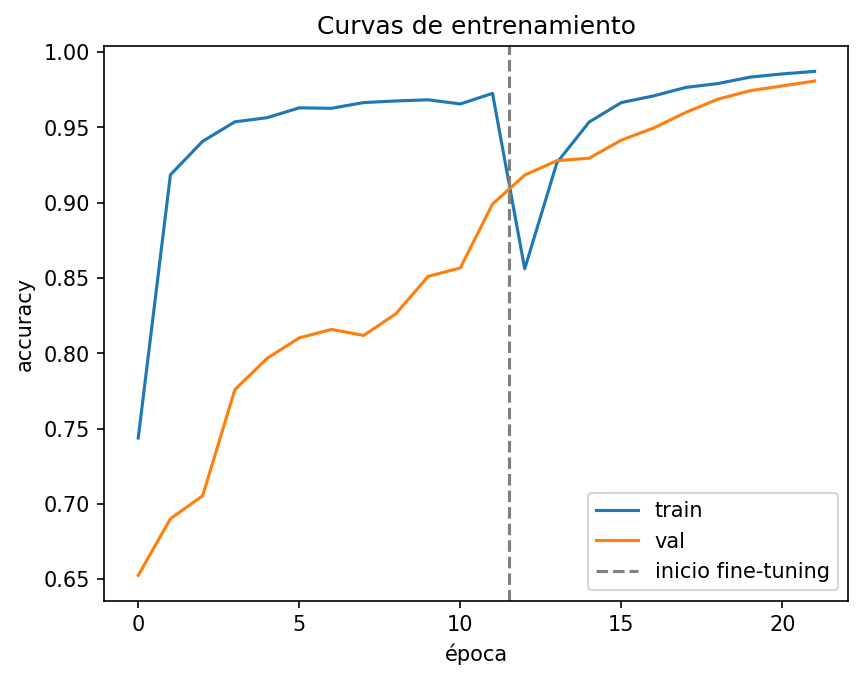
\includegraphics[width=0.92\columnwidth]{figuras/curvas.png}
\caption{Exactitud de entrenamiento y validación. La línea punteada marca el inicio del ajuste fino.}
\label{fig:curvas}
\end{figure}

\subsection{Desempeño del modelo cuantizado}

Sobre las 1237 imágenes de prueba, el modelo \texttt{.tflite} obtuvo una exactitud de 96,9~\% y un F1 macro de 0,969 (Tabla~\ref{tab:clases}), lo que confirma H1. La matriz de confusión (Fig.~\ref{fig:cm}) muestra que el billete de S/~10 es el más difícil: su exhaustividad es de 92,7~\%, y se confundió 12 veces con S/~20 y 9 veces con S/~50. Las demás confusiones no superan 4 casos por par de clases.

\begin{table}[!t]
\caption{Métricas por clase del modelo cuantizado (conjunto de prueba)}
\label{tab:clases}
\centering
\footnotesize
\begin{tabular}{|l|r|r|r|r|}
\hline
\textbf{Clase} & \textbf{Precisión} & \textbf{Exhaust.} & \textbf{F1} & \textbf{Imágenes} \\
\hline
S/~10 & 98,7~\% & 92,7~\% & 95,6~\% & 316 \\
S/~20 & 95,7~\% & 99,2~\% & 97,4~\% & 383 \\
S/~50 & 96,0~\% & 99,2~\% & 97,5~\% & 360 \\
S/~100 & 98,8~\% & 94,9~\% & 96,9~\% & 178 \\
\hline
Promedio macro & 97,3~\% & 96,5~\% & 96,9~\% & 1237 \\
\hline
\multicolumn{4}{|l|}{\textbf{Exactitud global}} & \textbf{96,9~\%} \\
\hline
\end{tabular}
\end{table}

\begin{figure}[!t]
\centering
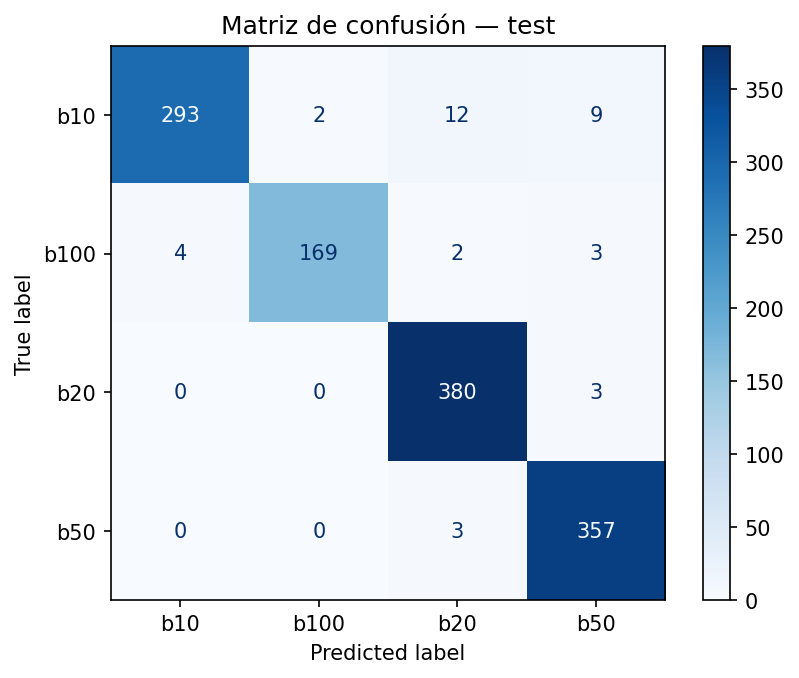
\includegraphics[width=0.85\columnwidth]{figuras/cm_test.png}
\caption{Matriz de confusión del modelo cuantizado en el conjunto de prueba (1237 imágenes). Filas: clase real; columnas: clase predicha, en orden alfabético de etiqueta.}
\label{fig:cm}
\end{figure}

\subsection{Efecto del umbral de confianza}

La Tabla~\ref{tab:umbral} resume el comportamiento con $\tau=0{,}85$. En el conjunto de prueba la aplicación habla en el 94,3~\% de los casos y solo el 0,77~\% de sus anuncios son erróneos, lo que confirma H2; en validación, los valores son 92,5~\% y 0,61~\%. Es decir, el umbral sacrifica alrededor de un 6~\% de respuestas a cambio de reducir los errores anunciados de 3,1~\% a menos de 1~\%.

\begin{table}[!t]
\caption{Resumen de resultados con umbral $\tau=0{,}85$}
\label{tab:umbral}
\centering
\footnotesize
\begin{tabular}{|l|r|r|}
\hline
\textbf{Métrica} & \textbf{Prueba} & \textbf{Validación} \\
\hline
Imágenes & 1237 & 1249 \\
Exactitud (sin umbral) & 96,9~\% & 97,3~\% \\
F1 macro & 0,969 & 0,973 \\
Cobertura (habla) & 94,3~\% & 92,5~\% \\
Error en los anuncios & 0,77~\% & 0,61~\% \\
\hline
Tamaño del modelo & \multicolumn{2}{c|}{1,13~MB} \\
\hline
\end{tabular}
\end{table}

\subsection{Aplicación desarrollada}

La Fig.~\ref{fig:app} muestra la aplicación funcionando en un teléfono Android. Tiene siete pantallas: inicio de sesión y registro, menú, Reconocer, Sumador, Historial, Ajustes y Ayuda. En la prueba funcional reconoció un billete de S/~20 de la familia antigua, doblado y sobre un fondo con estampado, y lo anunció por voz. El APK de producción para arquitecturas ARM64 pesa 27,1~MB (22,1~MB para ARMv7), por lo que cumple RNF3. Las pruebas unitarias de conversión de montos a palabras pasaron y el análisis estático no reportó problemas.

\begin{figure}[!t]
\centering
\begin{tabular}{@{}c@{\hspace{3mm}}c@{}}
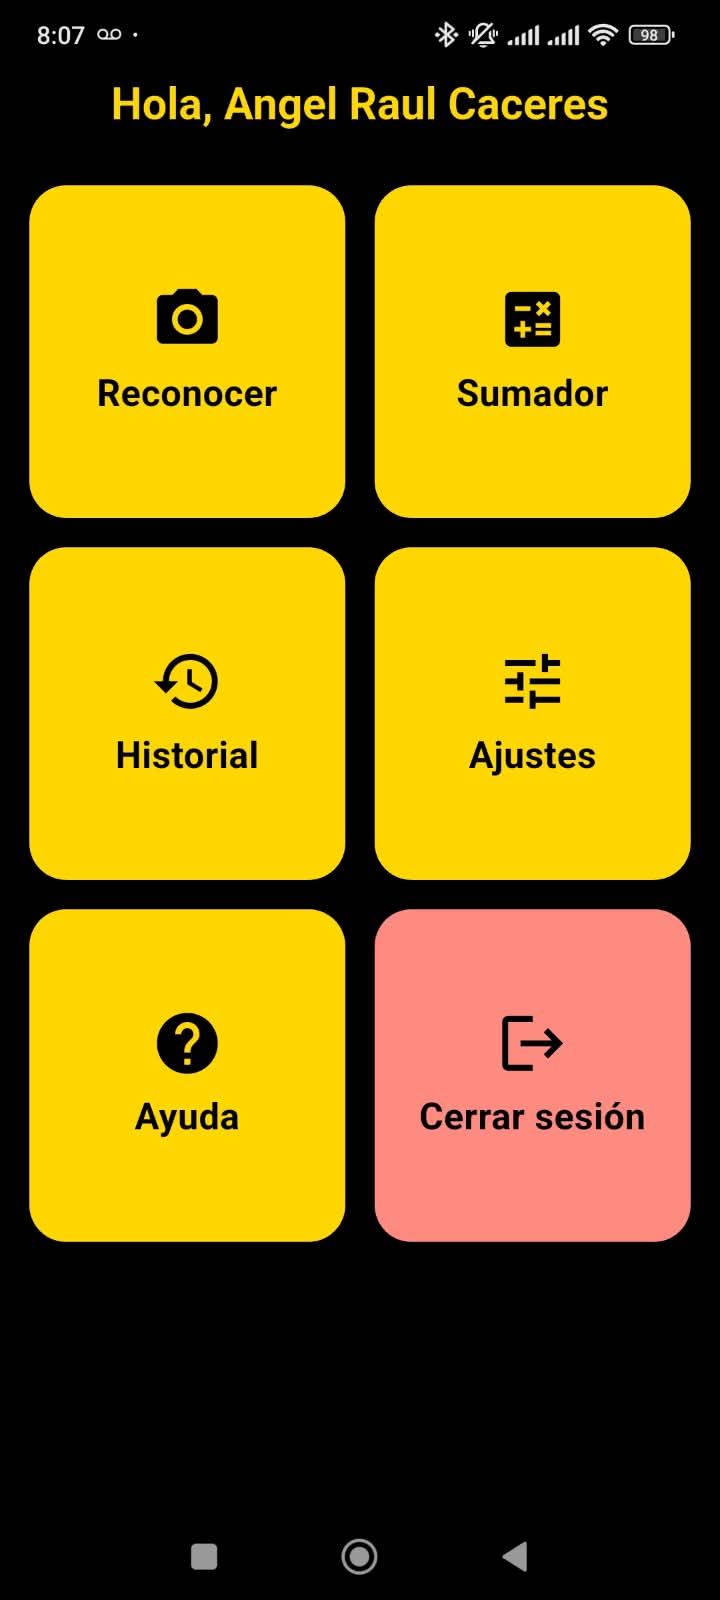
\includegraphics[width=0.4\columnwidth]{figuras/menu_principal.jpg} &
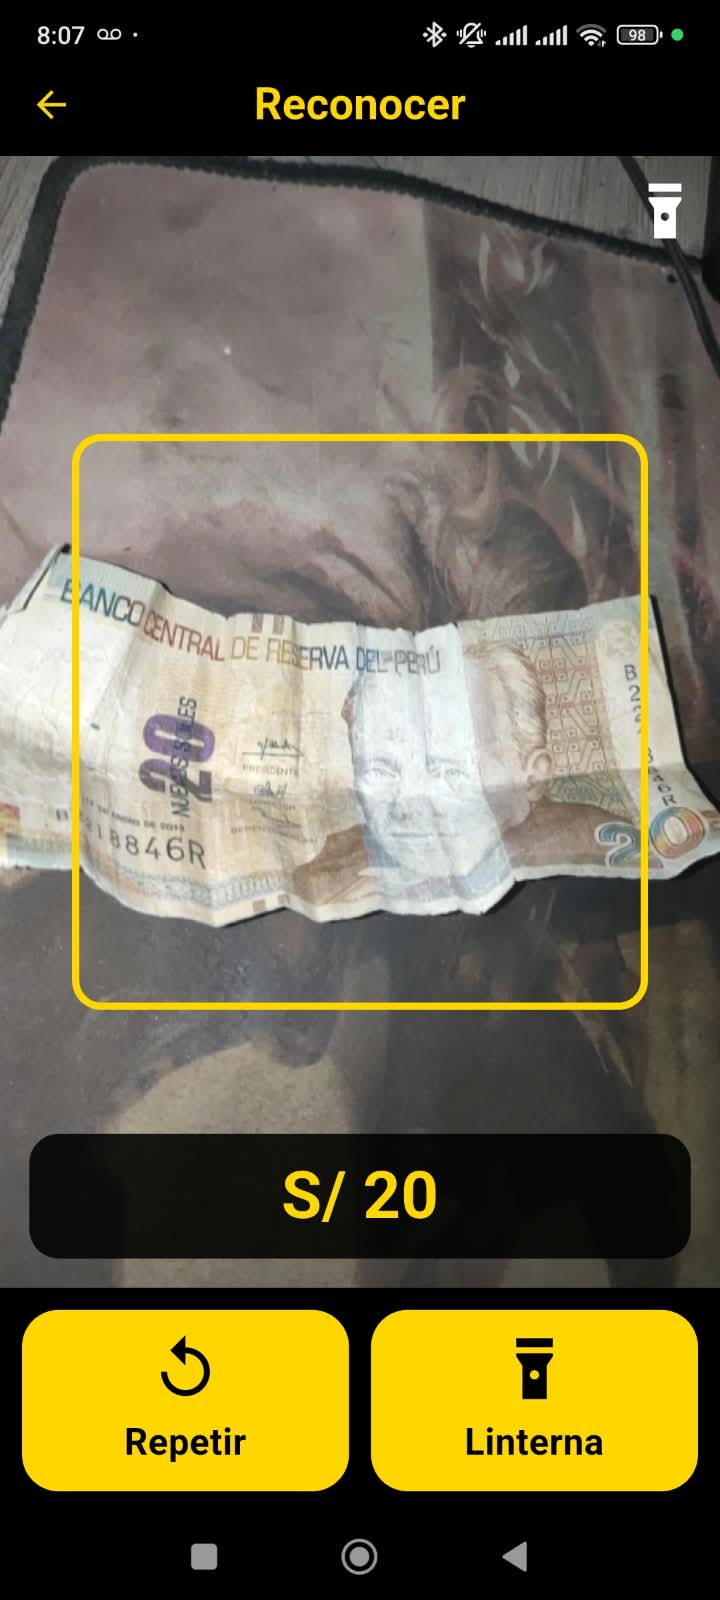
\includegraphics[width=0.4\columnwidth]{figuras/reconocer_billete_20.jpg} \\
\footnotesize (a) & \footnotesize (b)
\end{tabular}
\caption{Aplicación en un teléfono Android: (a) menú principal accesible; (b) reconocimiento de un billete de S/~20.}
\label{fig:app}
\end{figure}

\subsection{Muestra externa sin etiquetas}

En la Fig.~\ref{fig:ejemplos}, de 12 imágenes de la carpeta de prueba original, el modelo acertó 10. Los dos errores (un S/~100 de la familia nueva clasificado como S/~50, con 54~\% de confianza, y un S/~10 de la familia antigua clasificado como S/~20, con 73~\%) quedaron por debajo del umbral, por lo que la aplicación habría guardado silencio. Con $\tau=0{,}85$ habló en 8 de los 12 casos, sin errores. La muestra es pequeña, pero sugiere que fuera de la partición original la confianza baja y la exactitud real es menor que la medida en prueba.

\begin{figure*}[!t]
\centering
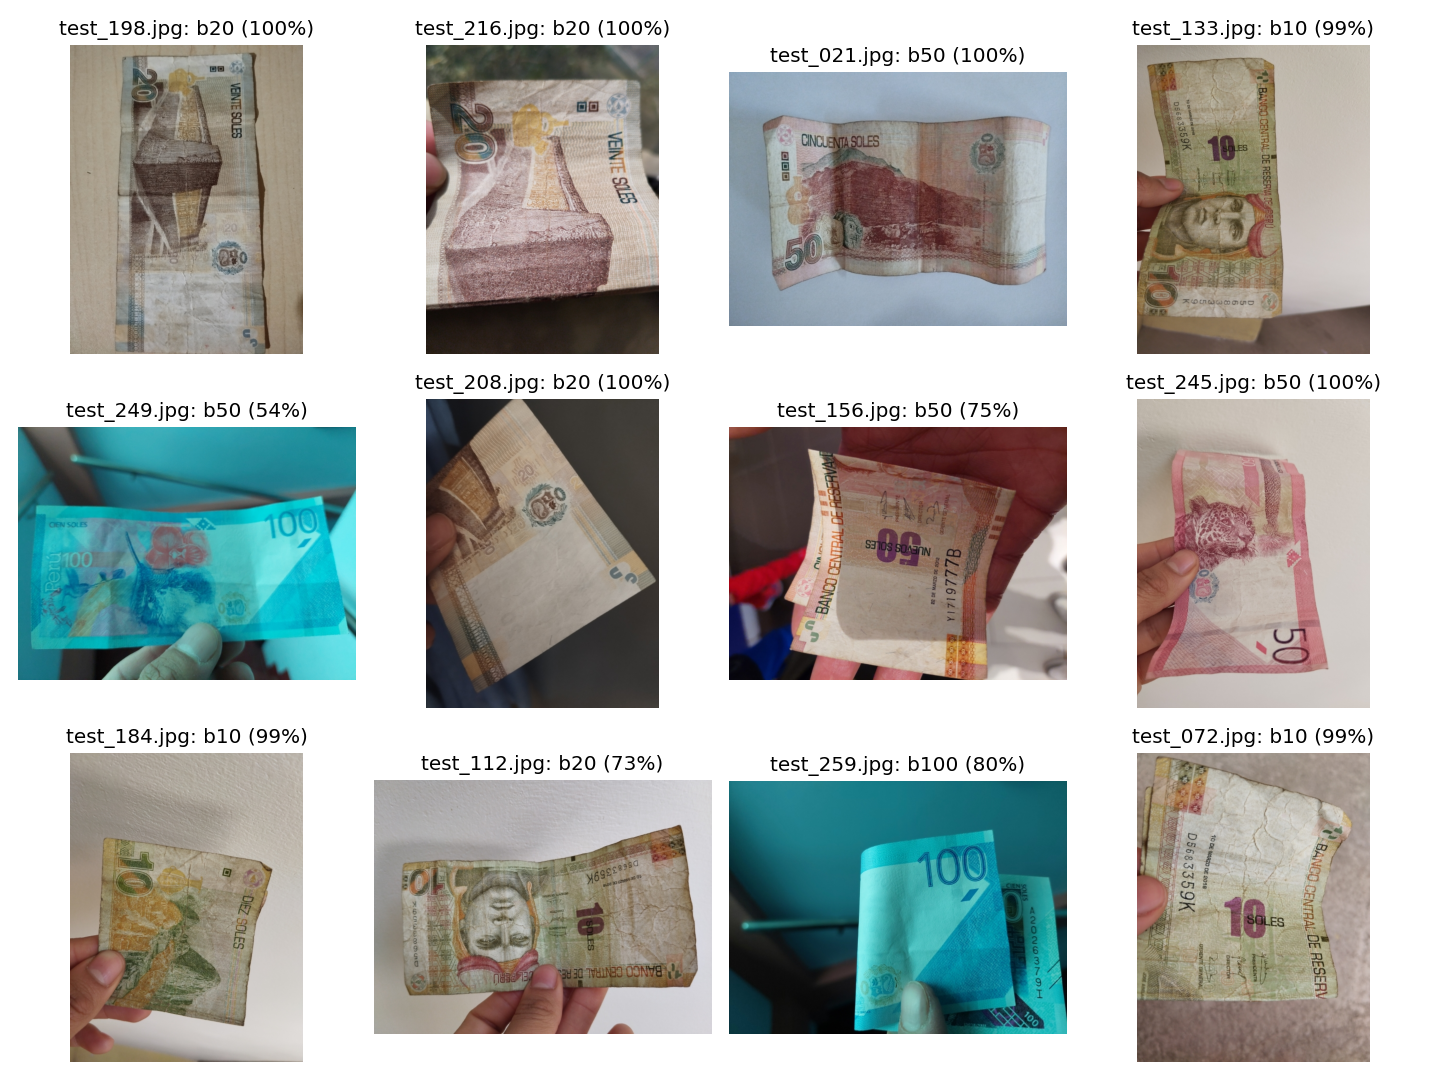
\includegraphics[width=0.64\textwidth]{figuras/ejemplos_testing_set.png}
\caption{Predicciones del modelo (clase y confianza) sobre 12 imágenes de la carpeta de prueba sin etiquetas del conjunto de datos.}
\label{fig:ejemplos}
\end{figure*}

\section{Discusión}

\subsection{Aporte central}

Hasta donde los autores conocen, este es uno de los primeros trabajos que convierte el conjunto de billetes peruanos de~\cite{caytuiro2023} en un sistema completo y utilizable: un modelo de 1,13~MB que corre sin conexión dentro de una aplicación accesible. El aporte no es solo la exactitud, sino el diseño orientado al usuario: preferir el silencio a un anuncio dudoso, hablar de forma pausada y en palabras, y ofrecer funciones de uso diario como el sumador con vuelto.

\subsection{Comparación con otros trabajos}

La Tabla~\ref{tab:comp} compara este trabajo con proyectos similares. Los sistemas basados en YOLO~\cite{mushtaq2025,ghanem2025,shreya2025} reportan métricas iguales o superiores, pero en general no evalúan su funcionamiento en un teléfono, y ninguno cubre el sol peruano. Este trabajo usa un clasificador más simple que un detector, lo que reduce el tamaño del modelo y el costo de inferencia, a cambio de reconocer un solo billete a la vez.

\begin{table*}[!t]
\caption{Comparación con trabajos relacionados}
\label{tab:comp}
\centering
\footnotesize
\begin{tabular}{|l|l|l|l|c|c|}
\hline
\textbf{Trabajo} & \textbf{Moneda} & \textbf{Modelo} & \textbf{Resultado reportado} & \textbf{En teléfono} & \textbf{Voz} \\
\hline
Caytuiro-Silva \emph{et al.} (2023)~\cite{caytuiro2023} & Sol peruano & -- (solo conjunto de datos) & -- & -- & -- \\
Mushtaq \emph{et al.} (2025)~\cite{mushtaq2025} & Rupia paquistaní & YOLOv8 & Exactitud 99,1~\% & N.R. & N.R. \\
Ghanem \emph{et al.} (2025)~\cite{ghanem2025} & Libra egipcia & YOLOv10 & F1 0,9715; mAP@0,5 0,9934 & No & N.R. \\
Shreya \emph{et al.} (2025)~\cite{shreya2025} & USD, EUR, BDT & YOLOv8n modificado & Exactitud 97,73~\% & N.R. & Sí \\
Oviedo \emph{et al.} (2022)~\cite{oviedo2022} & 17 monedas & MobileNetV2 (\emph{embeddings}) & Conjunto de datos abierto & -- & -- \\
\textbf{Este trabajo} & \textbf{Sol peruano} & \textbf{MobileNetV3-Small, TFLite} & \textbf{Exactitud 96,9~\%; F1 0,969} & \textbf{Sí} & \textbf{Sí} \\
\hline
\multicolumn{6}{l}{\scriptsize N.R.: no reportado.} \\
\end{tabular}
\end{table*}

\subsection{Alcance y limitaciones}

\begin{itemize}
\item El modelo reconoce cuatro denominaciones; todavía no incluye el billete de S/~200 ni las monedas.
\item No tiene una clase «fondo». Sin billete en la imagen, el modelo siempre elige alguna clase; el umbral y la votación reducen, pero no eliminan, los anuncios falsos.
\item Las particiones de prueba y validación provienen de la misma campaña de captura que el entrenamiento, por lo que las métricas son optimistas, como sugiere la muestra externa.
\item No se realizó una evaluación separada por condiciones de iluminación ni un estudio con usuarios con discapacidad visual.
\item No se midieron la latencia ni el consumo de energía en el dispositivo, y la versión para iOS no se probó en un equipo real.
\item La aplicación no detecta billetes falsos, y las cuentas son locales, sin sincronización.
\end{itemize}

\subsection{Trabajo futuro}

Se plantea: 1) ampliar el conjunto de datos con S/~200, monedas, una clase «fondo» y una clase para el lado del escudo de las monedas, que es igual en todas las denominaciones; 2) construir un conjunto de prueba independiente, separado por condiciones de iluminación (luz natural, interior, poca luz, contraluz y linterna); 3) realizar un estudio con usuarios ciegos y de baja visión, midiendo tasa de éxito, tiempo por billete y usabilidad (por ejemplo, con la escala SUS); 4) evaluar detectores ligeros tipo YOLO para reconocer varios billetes a la vez; y 5) medir latencia y consumo, y probar delegados de GPU.

\section{Conclusiones}

Se desarrolló Billetes Perú, una aplicación móvil accesible que reconoce billetes peruanos en el dispositivo y comunica su valor con voz con estilo de dictado, tonos y vibración. Un modelo MobileNetV3-Small cuantizado de 1,13~MB alcanzó 96,9~\% de exactitud en 1237 imágenes de prueba, lo que confirma H1, y el umbral de confianza de 0,85 mantuvo los anuncios erróneos en 0,77~\%, lo que confirma H2. La aplicación funciona sin internet en un teléfono Android e integra reconocimiento, sumador con vuelto, historial, cuentas y ajustes de accesibilidad. Los resultados muestran que es viable una herramienta de bajo costo y sin conexión para la autonomía financiera de las personas con discapacidad visual en el Perú, aunque se requieren pruebas por iluminación y con usuarios reales antes de su uso cotidiano.

\section*{Agradecimientos}

Los autores agradecen a Caytuiro-Silva \emph{et al.} por publicar abiertamente el conjunto de datos de billetes peruanos utilizado en este trabajo.

\begin{thebibliography}{00}
\bibitem{who2019} World Health Organization, \emph{World Report on Vision}. Geneva, Switzerland: WHO, 2019.
\bibitem{inei2019} Instituto Nacional de Estadística e Informática, \emph{Perú: Perfil Sociodemográfico de la Población con Discapacidad, 2017}. Lima, Perú: INEI, 2019.
\bibitem{bcrp2021} Banco Central de Reserva del Perú, \emph{Revista Moneda}, no.~187, Lima, Perú, 2021. [Online]. Available: \url{https://www.bcrp.gob.pe/docs/Publicaciones/Revista-Moneda/moneda-187/moneda-187-10.pdf}
\bibitem{caytuiro2023} N.~E. Caytuiro-Silva, J.~M. Peña-Alejandro, E.~G. Castro-Gutierrez, J.~Sulla-Torres, and B.~Maraza-Quispe, ``Annotated Peruvian banknote dataset for currency recognition and classification,'' \emph{Data in Brief}, vol.~51, Art.~no.~109715, 2023, doi: 10.1016/j.dib.2023.109715.
\bibitem{mendeley2023} N.~E. Caytuiro-Silva \emph{et al.}, ``Peruvian Banknotes,'' Mendeley Data, V1, 2023, doi: 10.17632/22jmt8xhpn.1.
\bibitem{cashreader} Perkins School for the Blind, ``Cash Reader.'' [Online]. Available: \url{https://www.perkins.org/resource/cash-reader/}
\bibitem{mushtaq2025} A.~Mushtaq, H.~W. Khan, M.~Salman, F.~Abid, J.~Rasheed, and S.~Alsubai, ``Helping blind individuals: Pakistani currency recognition system for blind people using the YOLOv8 model,'' \emph{UPB Sci. Bull., Ser. C}, vol.~87, no.~4, pp.~139--156, 2025.
\bibitem{ghanem2025} A.~M. Ghanem \emph{et al.}, ``Recognizing Egyptian currency for people with visual impairment using deep learning models,'' \emph{Sci. Rep.}, vol.~15, Art.~no.~34288, 2025, doi: 10.1038/s41598-025-20646-x.
\bibitem{shreya2025} S.~A. Shreya, M.~A.~I. Siddique, and S.~Tasnim, ``Real-time currency detection and voice feedback for visually impaired individuals,'' arXiv:2510.20267, 2025.
\bibitem{oviedo2022} F.~Oviedo, S.~Vinnakota, E.~Seleznev, H.~Malhotra, S.~Shaikh, and J.~Lavista Ferres, ``BankNote-Net: Open dataset for assistive universal currency recognition,'' arXiv:2204.03738, 2022.
\bibitem{howard2019} A.~Howard \emph{et al.}, ``Searching for MobileNetV3,'' in \emph{Proc. IEEE/CVF Int. Conf. Comput. Vis. (ICCV)}, 2019, pp.~1314--1324.
\bibitem{yosinski2014} J.~Yosinski, J.~Clune, Y.~Bengio, and H.~Lipson, ``How transferable are features in deep neural networks?'' in \emph{Adv. Neural Inf. Process. Syst.}, vol.~27, 2014, pp.~3320--3328.
\bibitem{deng2009} J.~Deng, W.~Dong, R.~Socher, L.-J. Li, K.~Li, and L.~Fei-Fei, ``ImageNet: A large-scale hierarchical image database,'' in \emph{Proc. IEEE Conf. Comput. Vis. Pattern Recognit. (CVPR)}, 2009, pp.~248--255.
\bibitem{jacob2018} B.~Jacob \emph{et al.}, ``Quantization and training of neural networks for efficient integer-arithmetic-only inference,'' in \emph{Proc. IEEE/CVF Conf. Comput. Vis. Pattern Recognit. (CVPR)}, 2018, pp.~2704--2713.
\bibitem{abadi2016} M.~Abadi \emph{et al.}, ``TensorFlow: A system for large-scale machine learning,'' in \emph{Proc. 12th USENIX Symp. Operating Syst. Design Implement. (OSDI)}, 2016, pp.~265--283.
\bibitem{litert} Google, ``LiteRT overview,'' Google AI Edge. [Online]. Available: \url{https://ai.google.dev/edge/litert}
\bibitem{flutter} Google, ``Flutter documentation.'' [Online]. Available: \url{https://docs.flutter.dev/}
\bibitem{pedregosa2011} F.~Pedregosa \emph{et al.}, ``Scikit-learn: Machine learning in Python,'' \emph{J. Mach. Learn. Res.}, vol.~12, pp.~2825--2830, 2011.
\bibitem{wcag22} World Wide Web Consortium, ``Web Content Accessibility Guidelines (WCAG) 2.2,'' W3C Recommendation, Oct. 2023. [Online]. Available: \url{https://www.w3.org/TR/WCAG22/}
\end{thebibliography}

\end{document}
